\chapter{पर्यावरण रसायन और विषविज्ञान}\label{ch:b3:environmental-toxicology}

हर ग्रीष्म के अंत में उपग्रह बड़ी झीलों पर फैलते हरे भँवरों के चित्र लेते हैं:
शैवाल-प्रस्फुटन, जिन्हें खेतों से बहकर और नगरों से निकलकर आने वाले फ़ॉस्फ़ेट और नाइट्रेट पोषित करते हैं।
जब शैवाल मरकर नीचे बैठते हैं, तो उनका सड़ना गहरे जल की ऑक्सीजन को समाप्त कर देता है,
और मछलियाँ मर जाती हैं। रसायन उस शृंखला की प्रत्येक कड़ी को समझाता है, और
अनेक अन्य शृंखलाओं को भी: कुछ गैसें ग्रह को क्यों गर्म करती हैं और अन्य क्यों नहीं, स्वच्छ वायु में भी
वर्षा अम्लीय क्यों होती है, छिड़कने के बाद कोई पीड़कनाशी कहाँ पहुँचता है, और किसी
पदार्थ की कितनी मात्रा हानि पहुँचाती है। यह अध्याय साम्यों, बलगतिकी और
स्पेक्ट्रमिकी को वायुमंडल, प्राकृतिक जलों और मृदाओं पर लागू करता है, उनके बीच
प्रदूषकों का पीछा करता है, और उन संख्याओं के साथ समाप्त होता है जिन पर जोखिम मूल्यांकन
आधारित होते हैं।

\begin{recall}
प्रथम वर्ष के खंड ने अम्ल--क्षारक, अवक्षेपण और संकुलन
साम्य, विभव--pH आरेख, विभाजन गुणांक, अर्ध-आयु, संकट,
जोखिम और GHS प्रणाली प्रस्तुत की; विद्यालय के खंड ने \omterm{def:b3:environmental-toxicology:greenhouse}{ग्रीनहाउस गैसें}; द्वितीय वर्ष के खंड ने
हेनरी का नियम, आयनिक सामर्थ्य, सांख्यिकी, द्रव्यमान स्पेक्ट्रममिति और परमाण्वीय
स्पेक्ट्रममिति। \Cref{ch:b3:photochemistry} ने वायुमंडलीय प्रकाशरसायन का विवेचन किया,
\cref{ch:b3:group-theory-applied} और \cref{ch:b3:rovibrational-spectroscopy} ने
अवरक्त सक्रियता का, और \cref{ch:b3:surfaces-catalysis} ने \omterm{def:b3:surfaces-catalysis:adsorption}{अधिशोषण} का।
\end{recall}

\begin{omfigure}
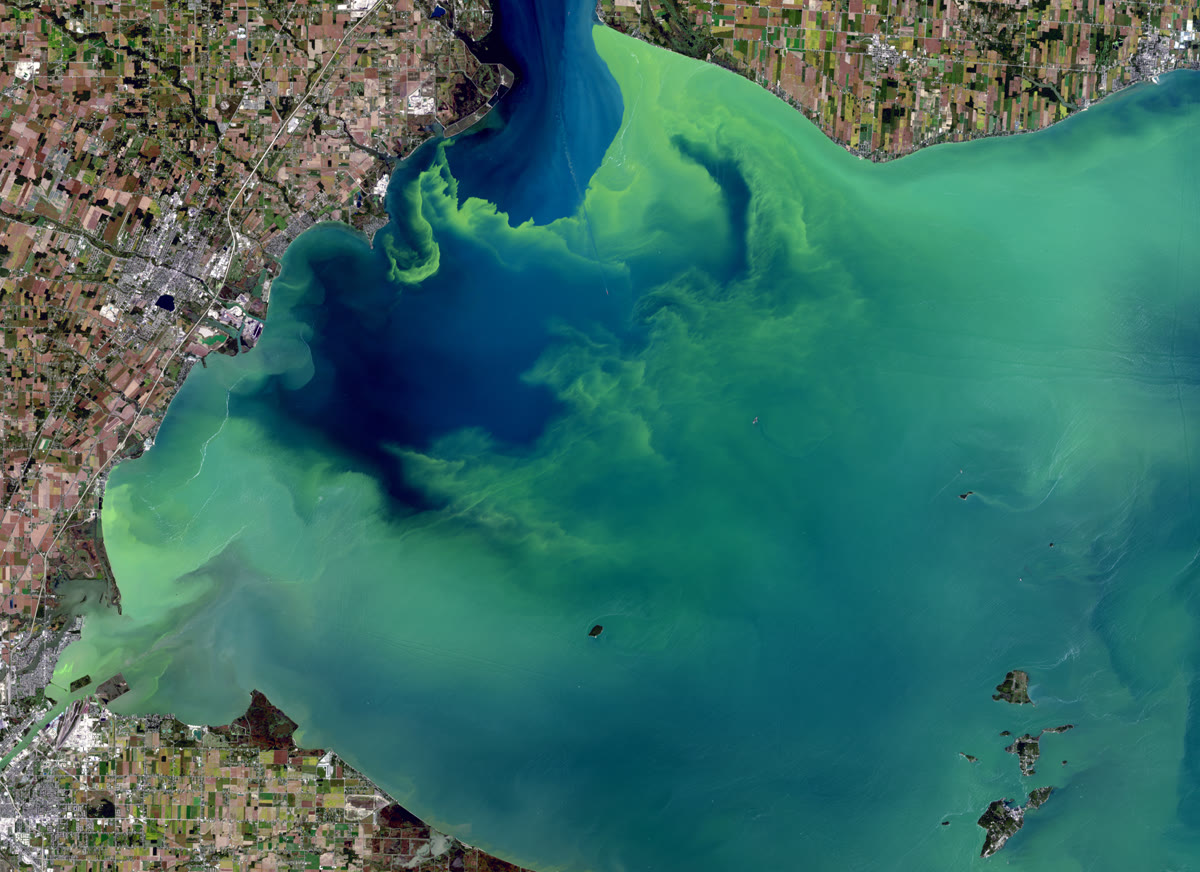
\includegraphics[width=0.62\linewidth]{images/book4/algal-bloom.jpg}

{\small एक बड़ी झील पर शैवाल-प्रस्फुटन, सितंबर के अंत में एक पृथ्वी-प्रेक्षण उपग्रह से
देखा गया: हरे भँवर सूक्ष्म शैवाल की सघन आबादियाँ हैं,
जिन्हें आसपास की कृषि-भूमि से आए पोषक तत्व पोषित करते हैं। चित्र: USGS और NASA, सार्वजनिक अधिकार-क्षेत्र।}
\end{omfigure}

\section{वायुमंडल}

\begin{definition}[ग्रीनहाउस गैसें]\label{def:b3:environmental-toxicology:greenhouse}
\emph{ग्रीनहाउस गैस}\index{ग्रीनहाउस गैस} पृथ्वी की सतह द्वारा उत्सर्जित विकिरण की
तरंगदैर्घ्यों पर अवरक्त विकिरण का अवशोषण और उत्सर्जन करती है, और
इस प्रकार निचले वायुमंडल को गर्म करती है। किसी गैस की \emph{वैश्विक तापन
क्षमता}\index{वैश्विक तापन क्षमता} (GWP), एक समय-क्षितिज पर,
सामान्यतः 100 वर्ष, एक किलोग्राम के उत्सर्जन के बाद उसके द्वारा रोकी गई ऊर्जा है,
एक किलोग्राम कार्बन डाइऑक्साइड के सापेक्ष।
\end{definition}

कोई अणु अवरक्त विकिरण का अवशोषण केवल उन कंपनों से करता है जो उसके
द्विध्रुव आघूर्ण को बदलते हैं (\cref{ch:b3:group-theory-applied})। डाइनाइट्रोजन और डाइऑक्सीजन,
समनाभिकीय द्विपरमाणुक, में ऐसा कोई कंपन नहीं होता और वे पारदर्शी हैं; आर्गन में कोई
कंपन होता ही नहीं। रैखिक और अध्रुवीय कार्बन डाइऑक्साइड में
\qty{15}{\micro\metre} के निकट एक \omterm{def:b3:group-theory-applied:activity}{अवरक्त-सक्रिय} बंकन विधा है, पृथ्वी के उत्सर्जन के ठीक मध्य में; जल, मेथेन
और नाइट्रस ऑक्साइड अनेक तरंगदैर्घ्यों पर अवशोषण करते हैं।

% ledger: atm:CO2.2025, atm:CH4.2025, atm:N2O.2025, gwp:CH4.fossil, gwp:CH4.nonfossil, gwp:N2O, life:CH4, life:N2O
2025 में वैश्विक माध्य मोल-अंश कार्बन डाइऑक्साइड के लिए \qty{425.6}{ppm}, मेथेन के लिए \qty{1936}{ppb} और
नाइट्रस ऑक्साइड के लिए \qty{338.9}{ppb} थे। हाइड्रॉक्सिल मूलकों द्वारा हटाई जाने वाली मेथेन, जिसका
जीवनकाल लगभग 12 वर्ष है, की GWP-100 27 से 30 है; केवल समतापमंडल में नष्ट होने वाली
नाइट्रस ऑक्साइड, जिसका जीवनकाल लगभग 109 वर्ष है, की 273। कार्बन डाइऑक्साइड का कोई
एकल जीवनकाल नहीं है: किसी उत्सर्जन का एक भाग सदियों तक वायु में रहता है।

\begin{definition}[वायु प्रदूषक]\label{def:b3:environmental-toxicology:pollutants}
\emph{कणिकीय पदार्थ}\index{कणिकीय पदार्थ} वायु में निलंबित ठोस और द्रव
कण हैं, जिन्हें वायुगतिकीय व्यास द्वारा वर्गीकृत किया जाता है (\qty{2.5}{\micro\metre} से छोटे
सूक्ष्म कण फेफड़ों में गहराई तक पहुँचते हैं)। \emph{अम्लीय
वर्षा}\index{अम्लीय वर्षा} वह वर्षा है जिसे सल्फ़र डाइऑक्साइड और नाइट्रोजन ऑक्साइडों से बने सल्फ़्यूरिक और
नाइट्रिक अम्ल स्वच्छ वर्षा से अधिक अम्लीय बना देते हैं।
\end{definition}

\begin{proposition}[स्वच्छ वर्षा का pH]\label{prop:b3:environmental-toxicology:rain-ph}
आज की वायु की कार्बन डाइऑक्साइड के साथ, और किसी अन्य चीज़ के साथ नहीं, साम्य में
वर्षा का pH लगभग 5.6 होता है।
\end{proposition}

\begin{proof}
% ledger: henry:CO2, pka4:H2CO3.1, pkw4:25C, const:atm
\emergencystretch=3em हेनरी का नियम $[\ce{CO2(aq)}] = K_Hp(\ce{CO2}) = \qty{3.4e-7}{mol.L^{-1}.Pa^{-1}} \times (425.6 \times 10^{-6} \times \qty{101325}{Pa}) = \qty{1.47e-5}{mol/L}$ देता है।
आवेश संतुलन $[\ce{H+}] = [\ce{HCO3-}] + 2[\ce{CO3^2-}] + [\ce{OH-}] \approx K_{a1}[\ce{CO2(aq)}]/[\ce{H+}] + K_w/[\ce{H+}]$ है, अतः
$[\ce{H+}]^2 = K_{a1}[\ce{CO2(aq)}] + K_w = 10^{-6.35} \times \num{1.47e-5} + 10^{-14} = \num{6.6e-12}$: $[\ce{H+}] = \qty{2.6e-6}{mol/L}$, pH 5.6।
\end{proof}

\emergencystretch=3em सल्फ़र-युक्त ईंधन जलाने से निकली सल्फ़र डाइऑक्साइड और गर्म दहन से निकले नाइट्रोजन
ऑक्साइड वायु में, हाइड्रॉक्सिल मूलकों द्वारा और मेघ-बूँदों में, ऑक्सीकृत होकर
सल्फ़्यूरिक और नाइट्रिक अम्ल बनते हैं, जो वर्षा को pH 4 और उससे नीचे तक ले आते हैं।
ईंधनों से सल्फ़र और निकास गैसों से नाइट्रोजन ऑक्साइड हटाने (उत्प्रेरकी
परिवर्तक, बिजलीघरों में अमोनिया अंतःक्षेपण) ने, जहाँ यह लागू किया गया, समस्या को काफ़ी हद तक हल कर दिया है।
भूमि के निकट ओज़ोन, जो सूर्य-प्रकाश के नाइट्रोजन ऑक्साइडों और
वाष्पशील कार्बनिक यौगिकों पर क्रिया करने से बनती है (\cref{ch:b3:photochemistry}), और
सूक्ष्म कण स्वास्थ्य के लिए मुख्य वायु प्रदूषक बने हुए हैं।

\section{प्राकृतिक जल}

\begin{omfigure}
\begin{tikzpicture}
\begin{axis}[name=a, width=0.48\linewidth, height=5.4cm, xmin=4, xmax=13, ymin=0, ymax=1.02,
  axis lines=left, xlabel={pH}, ylabel={घुले कार्बन का अंश},
  tick label style={font=\scriptsize}, label style={font=\small}]
\addplot[color=omDef, thick] table[x=pH, y=a0] {figdata/out/bachelor-3-carbonate-system.dat};
\addplot[color=omMeth, thick] table[x=pH, y=a1] {figdata/out/bachelor-3-carbonate-system.dat};
\addplot[color=omThm, thick] table[x=pH, y=a2] {figdata/out/bachelor-3-carbonate-system.dat};
\node[font=\scriptsize, omDef] at (axis cs:4.9,0.85) {$\ce{CO2(aq)}$};
\node[font=\scriptsize, omMeth] at (axis cs:8.3,0.88) {$\ce{HCO3-}$};
\node[font=\scriptsize, omThm] at (axis cs:12.1,0.85) {$\ce{CO3^2-}$};
\draw[black!30, dashed] (axis cs:6.35,0) -- (axis cs:6.35,0.5) (axis cs:10.33,0) -- (axis cs:10.33,0.5);
\end{axis}
\begin{axis}[at={(a.east)}, anchor=west, xshift=1.4cm, width=0.48\linewidth, height=5.4cm,
  xmin=0, xmax=2000, ymin=5.2, ymax=6.2, axis lines=left,
  xlabel={वायु में $\ce{CO2}$ / ppm}, ylabel={वर्षा का pH},
  tick label style={font=\scriptsize}, label style={font=\small},
  scaled x ticks=false, xticklabel style={/pgf/number format/1000 sep={}}]
\addplot[color=omDef, thick] table[x=ppm, y=pH] {figdata/out/bachelor-3-carbonate-system-b.dat};
\draw[black!35, dashed] (axis cs:425.6,5.2) -- (axis cs:425.6,5.59);
\node[font=\scriptsize, anchor=west] at (axis cs:470,5.63) {आज: 5.6};
\end{axis}
\end{tikzpicture}

{\small बाएँ: \qty{25}{\celsius} पर pH के विरुद्ध घुले अकार्बनिक कार्बन का उसके तीन रूपों में वितरण,
जो $\mathrm pK_{a1} = 6.35$ और $\mathrm pK_{a2} = 10.33$ पर एक-दूसरे को काटते हैं। दाएँ: केवल कार्बन डाइऑक्साइड के साथ
साम्य में वर्षा का pH, वायु में उसके मोल-अंश के विरुद्ध।}
\end{omfigure}

\begin{proposition}[कार्बोनेट अंश]\label{prop:b3:environmental-toxicology:carbonate-fractions}
$C_T$ को कुल घुला अकार्बनिक कार्बन लेते हुए,
$[\ce{CO2(aq)}] = C_Th^2/D$, $[\ce{HCO3-}] = C_TK_{a1}h/D$, $[\ce{CO3^2-}] = C_TK_{a1}K_{a2}/D$, जहाँ $h = [\ce{H+}]$ और $D = h^2 + K_{a1}h + K_{a1}K_{a2}$।
\end{proposition}

\begin{proof}
दोनों अम्लता स्थिरांकों से,
\[
  [\ce{HCO3-}] = \frac{K_{a1}[\ce{CO2(aq)}]}{h}, \qquad [\ce{CO3^2-}] = \frac{K_{a2}[\ce{HCO3-}]}{h} = \frac{K_{a1}K_{a2}[\ce{CO2(aq)}]}{h^2}.
\]
इनका योग $C_T = [\ce{CO2(aq)}]\,D/h^2$ है; प्रत्येक रूप को $C_T$ से भाग देने पर अंश मिलते हैं।
\end{proof}

\begin{definition}[क्षारीयता]\label{def:b3:environmental-toxicology:alkalinity}
किसी जल की \emph{क्षारीयता}\index{क्षारीयता} प्रबल अम्ल को उदासीन करने की
उसकी क्षमता है, जिसे कार्बोनिक अम्ल के अंत्य बिंदु (लगभग pH
4.5) तक अनुमापन से मापा जाता है और प्रति लीटर $\ce{H+}$ के मोलों में व्यक्त किया जाता है।
\end{definition}

\begin{proposition}[कार्बोनेट क्षारीयता]\label{prop:b3:environmental-toxicology:alkalinity}
जिस जल के क्षारक कार्बोनेट स्पीशीज़ और हाइड्रॉक्साइड हों, उसमें
$\mathrm{Alk} = [\ce{HCO3-}] + 2[\ce{CO3^2-}] + [\ce{OH-}] - [\ce{H+}]$; यह प्रबल-क्षारक धनायनों के आवेशों के
प्रबल-अम्ल ऋणायनों के आवेशों पर आधिक्य के बराबर है, और वायु के साथ कार्बन डाइऑक्साइड
के विनिमय से नहीं बदलती।
\end{proposition}

\begin{proof}
कार्बोनिक अम्ल के अंत्य बिंदु तक अनुमापन प्रत्येक $\ce{HCO3-}$ को $\ce{CO2}$ में बदलता है (प्रत्येक एक $\ce{H+}$),
प्रत्येक $\ce{CO3^2-}$ को $\ce{CO2}$ में (दो), प्रत्येक $\ce{OH-}$ को जल में (एक), जबकि पहले से उपस्थित मुक्त $\ce{H+}$
विपक्ष में गिना जाता है: कथित योग। जल का आवेश संतुलन,
$\ce{Na+}$, $\ce{Ca^2+}$\dots{} और $\ce{Cl-}$, $\ce{SO4^2-}$\dots के साथ, पुनर्व्यवस्थित होकर उसी योग को देता है, जो प्रबल विद्युत-अपघट्यों के $\sum z_i c_i$(धनायन) $-$ $\sum z_jc_j$(ऋणायन)
के बराबर है। $\ce{CO2}$ जोड़ने या हटाने से इनमें से कोई आयन नहीं बदलता।
\end{proof}

\begin{definition}[महासागर अम्लीकरण]\label{def:b3:environmental-toxicology:acidification}
\emph{महासागर अम्लीकरण}\index{महासागर अम्लीकरण} समुद्री जल के pH की वह कमी है
जो वायु से कार्बन डाइऑक्साइड ग्रहण करने पर होती है। किसी कार्बोनेट खनिज की \emph{संतृप्ति
अवस्था}\index{संतृप्ति अवस्था}
$\Omega = [\ce{Ca^2+}][\ce{CO3^2-}]/K_{sp}$ है: 1 से ऊपर खनिज बन सकता है, 1 से नीचे वह घुलने की प्रवृत्ति रखता है।
\end{definition}

घुली कार्बन डाइऑक्साइड कार्बोनेट आयनों को हाइड्रोजनकार्बोनेट में बदलती है, $\ce{CO2 + CO3^2- + H2O -> 2HCO3-}$,
जिससे pH और $\Omega$ घटते हैं: खोलों और प्रवाल-कंकालों का निर्माण कठिन हो जाता है। (समुद्री
जल में स्थिरांक आभासी होते हैं, लवणीय माध्यम में मापे गए, और
इस अध्याय के मीठे-जल मानों से भिन्न होते हैं।)

\begin{definition}[जल की कठोरता]\label{def:b3:environmental-toxicology:hardness}
किसी जल की \emph{कठोरता}\index{जल की कठोरता} उसके कैल्सियम और मैग्नीशियम आयनों की
कुल सांद्रता है, जिसे प्रायः कैल्सियम कार्बोनेट के उस द्रव्यमान के रूप में व्यक्त किया जाता है
जिसमें मोलों की उतनी ही संख्या हो, mg/L में।
\end{definition}

\begin{definition}[ऑक्सीजन माँग]\label{def:b3:environmental-toxicology:oxygen-demand}
किसी जल की \emph{जैवरासायनिक ऑक्सीजन माँग}\index{जैवरासायनिक ऑक्सीजन माँग} (BOD)
प्रति लीटर डाइऑक्सीजन का वह द्रव्यमान है जिसे सूक्ष्मजीव उसके
कार्बनिक पदार्थ को अँधेरे में, एक निर्दिष्ट समय में (\qty{20}{\celsius} पर पाँच दिन, $\mathrm{BOD_5}$ के लिए), ऑक्सीकृत करते हुए उपभुक्त करते हैं। उसकी
\emph{रासायनिक ऑक्सीजन माँग}\index{रासायनिक ऑक्सीजन माँग} (COD) डाइऑक्सीजन का वह
द्रव्यमान है जो उसके कार्बनिक पदार्थ को रासायनिक रूप से ऑक्सीकृत करने में उपभुक्त
डाइक्रोमेट के तुल्य है।
\end{definition}

\begin{proposition}[BOD वक्र]\label{prop:b3:environmental-toxicology:bod}
यदि जैवनिम्नीकरणीय कार्बनिक पदार्थ दर
स्थिरांक $k$ के साथ प्रथम-कोटि बलगतिकी से उपभुक्त होता है, तो समय $t$ के बाद प्रयुक्त ऑक्सीजन $\mathrm{BOD}_t = L_0(1 - \eu^{-kt})$ है, जहाँ $L_0$ अंतिम BOD है।
\end{proposition}

\begin{proof}
शेष माँग $L$ समीकरण $\dd L/\dd t = -kL$ का पालन करती है, अतः $L = L_0\eu^{-kt}$; प्रयुक्त ऑक्सीजन वह है जो जा चुकी है,
$L_0 - L$।
\end{proof}

\begin{omfigure}
\begin{tikzpicture}
\begin{axis}[name=a, width=0.48\linewidth, height=5.2cm, xmin=0, xmax=30, ymin=0, ymax=270,
  axis lines=left, xlabel={समय / दिन}, ylabel={BOD / \unit{mg.L^{-1}}},
  tick label style={font=\scriptsize}, label style={font=\small}]
\addplot[color=omDef, thick] table[x=t, y=bod] {figdata/out/bachelor-3-bod.dat};
\draw[black!35, dashed] (axis cs:0,250) -- (axis cs:30,250);
\draw[black!35, dashed] (axis cs:5,0) -- (axis cs:5,170.8);
\node[font=\scriptsize, anchor=west] at (axis cs:5.6,140) {$\mathrm{BOD_5}$};
\node[font=\scriptsize, anchor=north east] at (axis cs:30,246) {$L_0$};
\end{axis}
\begin{axis}[at={(a.east)}, anchor=west, xshift=1.4cm, width=0.48\linewidth, height=5.2cm,
  xmin=0, xmax=15, ymin=0, ymax=10, axis lines=left,
  xlabel={अनुप्रवाह समय / दिन}, ylabel={घुली $\ce{O2}$ / \unit{mg.L^{-1}}},
  tick label style={font=\scriptsize}, label style={font=\small}]
\addplot[color=omThm, thick] table[x=t, y=O2] {figdata/out/bachelor-3-bod-b.dat};
\draw[black!35, dashed] (axis cs:0,9.1) -- (axis cs:15,9.1);
\node[font=\scriptsize, anchor=south east] at (axis cs:15,9.1) {सन्तृप्त};
\node[font=\scriptsize, anchor=north] at (axis cs:2.4,6.3) {क्रांतिक बिंदु};
\end{axis}
\end{tikzpicture}

{\small बाएँ: एक मॉडल मलजल की BOD, $L_0 = \qty{250}{mg/L}$ और $k = \qty{0.23}{d^{-1}}$: माँग का लगभग दो-तिहाई
भाग पाँच दिनों में प्रयुक्त होता है। दाएँ: किसी निकास-मुख के नीचे नदी में ऑक्सीजन का अवनमन
(स्ट्रीटर--फ़ेल्प्स मॉडल): आरंभ में कार्बनिक भार का अपघटन ऑक्सीजन को उससे तेज़ी से उपभुक्त करता है
जितनी तेज़ी से वायु उसे पुनः भरती है, जब तक कि लगभग 2.4 दिनों बाद कमी शिखर पर नहीं पहुँचती।}
\end{omfigure}

\begin{method}[COD का निर्धारण]\label{met:b3:environmental-toxicology:cod}
\begin{enumerate}
  \item नमूने के एक मापे गए आयतन को सल्फ़्यूरिक अम्ल में पोटैशियम
        डाइक्रोमेट की ज्ञात अधिक मात्रा के साथ, उत्प्रेरक के रूप में सिल्वर सल्फ़ेट और
        क्लोराइड को बाँधने के लिए मर्करी(II) सल्फ़ेट के साथ, पश्चवाहित कीजिए।
  \item शेष डाइक्रोमेट का फ़ेरोइन का उपयोग करते हुए आयरन(II) से अनुमापन कीजिए, और शुद्ध जल के साथ एक
        रिक्त (ब्लैंक) प्रयोग चलाइए।
  \item उपभुक्त डाइक्रोमेट, $\ce{O2}$ के तुल्य द्रव्यमान में बदला गया (एक
        $\ce{Cr2O7^2-}$ छह इलेक्ट्रॉन लेता है, जैसे 1.5 $\ce{O2}$ लेते), और नमूने के आयतन से भाग दिया गया,
        mg/L में COD है।
\end{enumerate}
\end{method}

\begin{definition}[सुपोषण]\label{def:b3:environmental-toxicology:eutrophication}
\emph{सुपोषण}\index{सुपोषण} किसी जलाशय का पोषक तत्वों से, मुख्यतः
फ़ॉस्फ़ोरस और नाइट्रोजन से, समृद्धीकरण है, जिससे शैवाल और पौधों की अत्यधिक वृद्धि होती है,
और फिर उनके सड़ने पर ऑक्सीजन की कमी।
\end{definition}

\begin{omfigure}
\begin{tikzpicture}[font=\scriptsize, >=Stealth,
  box/.style={draw, rounded corners, align=center, fill=omMeth!10, inner sep=3pt, minimum height=8mm}]
  \node[box] (f) at (-3.4,1.2) {खेत: उर्वरक,\\ खाद};
  \node[box] (t) at (-3.4,-0.4) {नगर: मलजल,\\ डिटर्जेंट};
  \node[box] (a) at (0,2.1) {वायुमंडल:\\ निक्षेपण (N)};
  \node[box, fill=omDef!12, minimum width=3.2cm, minimum height=1.7cm] (l) at (0.6,0.4) {झील का जल:\\ शैवाल बढ़ते हैं};
  \node[box, fill=black!8] (s) at (0.6,-1.6) {तलछट: P संचित,\\ अनॉक्सी होने पर मुक्त};
  \node[box] (o) at (4.0,0.4) {बहिर्वाह};
  \draw[->, thick] (f) -- node[above, sloped, pos=0.4] {अपवाह} (l);
  \draw[->, thick] (t) -- node[below, sloped] {N, P} (l);
  \draw[->, thick] (a) -- (l);
  \draw[->, thick] (l) -- node[left] {मृत शैवाल} (s);
  \draw[->, thick, dashed] (s.east) to[bend right=30] node[right] {P} (l.south east);
  \draw[->, thick] (l) -- (o);
\end{tikzpicture}

{\small किसी झील में और उसके भीतर पोषक तत्वों का प्रवाह। फ़ॉस्फ़ोरस, जो मीठे जल में प्रायः सीमाकारी
पोषक तत्व होता है, तलछट में संचित होता है और तल के ऑक्सीजनरहित होने पर जल में लौट आता है,
जो निवेश रोके जाने के बाद भी वर्षों तक प्रस्फुटन को बनाए रख सकता है।}
\end{omfigure}

शैवाल कार्बन, नाइट्रोजन और फ़ॉस्फ़ोरस को लगभग नियत अनुपातों में ग्रहण करते हैं;
उन आवश्यकताओं के सापेक्ष जो भी पोषक तत्व कम हो, वही उनकी वृद्धि को सीमित करता है। अधिकांश
झीलों में यह फ़ॉस्फ़ोरस है, इसीलिए फ़ॉस्फ़ेट डिटर्जेंटों से और
उपचारित मलजल से हटाए गए; अनेक तटीय समुद्रों में यह नाइट्रोजन है।

\begin{definition}[स्पीशीज़-वितरण]\label{def:b3:environmental-toxicology:speciation}
किसी नमूने में किसी तत्व का \emph{रासायनिक स्पीशीज़-वितरण}\index{रासायनिक स्पीशीज़-वितरण}
उसकी मात्रा का उसके रासायनिक रूपों में वितरण है: ऑक्सीकरण
अवस्थाएँ, संकुल, कार्बधात्विक यौगिक, मुक्त और बद्ध स्पीशीज़।
\end{definition}

विषाक्तता स्पीशीज़-वितरण पर निर्भर करती है। जल में मुक्त अकार्बनिक पारा
तलछट में जीवाणुओं द्वारा मेथिलीकृत होकर मेथिलमर्करी बनता है, जो झिल्लियों को पार करता है,
प्रोटीनों के सल्फ़र से बँधता है और खाद्य शृंखलाओं में ऊपर की ओर सांद्रित होता है; आर्सेनिक,
आर्सेनाइट, As(III), के रूप में आर्सेनेट, As(V), की तुलना में कहीं अधिक विषैला है, और समुद्री भोजन में पाए जाने वाले
कार्बनिक रूपों में बहुत कम। केवल कुल सांद्रता बहुत कम बताती है।

\begin{method}[किसी जल में किसी धातु का स्पीशीज़-वितरण]\label{met:b3:environmental-toxicology:speciation}
\begin{enumerate}
  \item उपस्थित लिगैंडों (हाइड्रॉक्साइड, कार्बोनेट, क्लोराइड, सल्फ़ेट, कार्बनिक
        पदार्थ) को उनकी सांद्रताओं और pH के साथ सूचीबद्ध कीजिए।
  \item प्रथम वर्ष के खंड की तरह, संकुलन स्थिरांक और धातु का द्रव्यमान
        संतुलन लिखिए।
  \item मुक्त धातु आयन के लिए हल कीजिए, फिर प्रत्येक संकुल के लिए; pH के विरुद्ध या किसी
        लिगैंड सांद्रता के विरुद्ध अंश आलेखित कीजिए।
  \item विषैले या जैवउपलब्ध रूप (प्रायः मुक्त आयन) की तुलना कुल से कीजिए।
\end{enumerate}
\end{method}

\section{मृदाएँ और तलछट}

\begin{definition}[मृदाओं में शोषण]\label{def:b3:environmental-toxicology:soil}
किसी मृदा की \emph{धनायन विनिमय क्षमता}\index{धनायन विनिमय क्षमता}
विनिमेय धनायनों की वह मात्रा है जिसे वह प्रति इकाई द्रव्यमान, मृत्तिकाओं और कार्बनिक
पदार्थ पर, धारण कर सकती है। \emph{मृदा--जल वितरण गुणांक}\index{मृदा--जल वितरण गुणांक}
$K_d$ मृदा पर शोषित किसी पदार्थ की सांद्रता (प्रति किलोग्राम) का रंध्र-जल में उसकी
सांद्रता (प्रति लीटर) से अनुपात है; \emph{कार्बनिक-कार्बन विभाजन गुणांक}\index{कार्बनिक-कार्बन विभाजन गुणांक}
$K_{oc} = K_d/f_{oc}$ है, जहाँ $f_{oc}$ कार्बनिक कार्बन का द्रव्यमान-अंश है।
\end{definition}

उदासीन कार्बनिक यौगिक मुख्यतः मृदा के कार्बनिक पदार्थ पर शोषित होते हैं, इसलिए $K_{oc}$ एक मृदा से
दूसरी मृदा में $K_d$ की तुलना में बहुत कम बदलता है। छोटे $K_d$ वाला यौगिक जल के साथ चलता है
और भूजल तक पहुँच सकता है (निक्षालन); बड़े $K_d$ वाला यौगिक सतह के निकट रहता है,
उन कणों से बँधा जिन्हें अपरदन नदियों और झीलों में ले जा सकता है।

\section{प्रदूषकों की नियति}

\begin{definition}[ऑक्टेनॉल--जल विभाजन गुणांक]\label{def:b3:environmental-toxicology:kow}
किसी पदार्थ का \emph{ऑक्टेनॉल--जल विभाजन गुणांक}\index{ऑक्टेनॉल--जल विभाजन गुणांक}
$K_{ow}$ ऑक्टेन-1-ऑल और जल में उसकी साम्य सांद्रताओं का
अनुपात है; यह वसीय ऊतकों और कार्बनिक पदार्थ के प्रति उसकी बंधुता को
मापता है।
\end{definition}

% ledger: logkow:DDT, logkow:benzene, logkow:atrazine, logkow:PCB153
बेंज़ीन का $\log K_{ow} = 2.13$ है, शाकनाशी एट्राज़ीन का 2.61, एक हेक्साक्लोरीनित PCB का 6.67 और
DDT का 6.91: अंतिम दो जल की तुलना में वसा में करोड़ों गुना बेहतर
घुलते हैं।

\begin{definition}[जैवसंचयन]\label{def:b3:environmental-toxicology:bio}
\emph{जैवसांद्रण गुणक}\index{जैवसांद्रण गुणक} (BCF) स्थायी अवस्था में किसी जीव में
सांद्रता का आसपास के जल में सांद्रता से अनुपात है, जब ग्रहण
केवल जल से हो। \emph{जैवसंचयन}\index{जैवसंचयन}
सभी मार्गों से, भोजन सहित, किसी जीव में होने वाला संचय है;
\emph{जैवआवर्धन}\index{जैवआवर्धन} किसी खाद्य शृंखला में ऊपर की ओर
शिकार से शिकारी तक सांद्रता में वृद्धि है।
\end{definition}

\begin{proposition}[BCF और $K_{ow}$]\label{prop:b3:environmental-toxicology:bcf-kow}
उन उदासीन कार्बनिक पदार्थों के लिए जिनका उपापचय नहीं होता, मछली में $\log\mathrm{BCF}$
लगभग $\log K_{ow}$ का रैखिक फलन होता है, 1 के निकट ढलान के साथ, $\log K_{ow}$ के लगभग 6 तक;
उससे ऊपर ग्रहण धीमा हो जाता है और संबंध समतल हो जाता है (आनुभविक समाश्रयण)।
\admitted
\end{proposition}

\begin{definition}[चिरस्थायी कार्बनिक प्रदूषक]\label{def:b3:environmental-toxicology:pop}
\emph{चिरस्थायी कार्बनिक प्रदूषक}\index{चिरस्थायी कार्बनिक प्रदूषक} ऐसा
कार्बनिक पदार्थ है जो निम्नीकरण का प्रतिरोध करता है, जैवसंचित होता है, विषैला है और
अपने स्रोतों से दूर तक परिवहित होता है, जैसे DDT, PCB और डाइऑक्सिन।
\end{definition}

\begin{proposition}[विभागों के बीच साम्य वितरण]\label{prop:b3:environmental-toxicology:level-one}
किसी पदार्थ का द्रव्यमान $M$, जो साम्य पर (एक ``स्तर I'' मॉडल) जल
(आयतन $V_w$), वायु ($V_a$), तलछट ठोसों ($m_s$) और मछली ($m_f$) में वितरित हो, जल-सांद्रता
$C_w = M/(V_w + K_{aw}V_a + K_{sw}m_s + K_{fw}m_f)$ रखता है, जहाँ $K$ जल के सापेक्ष विभाजन गुणांक हैं;
प्रत्येक विभाग में द्रव्यमान उसका पद गुणा $C_w$ है।
\end{proposition}

\begin{proof}
साम्य पर $C_a = K_{aw}C_w$, $C_s = K_{sw}C_w$ (प्रति किलोग्राम), $C_f = K_{fw}C_w$। द्रव्यमान संतुलन
$M = C_wV_w + C_aV_a + C_sm_s + C_fm_f = C_w(V_w + K_{aw}V_a + K_{sw}m_s + K_{fw}m_f)$ है; भाग देने पर $C_w$ मिलता है।
\end{proof}

\begin{omfigure}
\begin{tikzpicture}[font=\scriptsize, >=Stealth,
  comp/.style={draw, rounded corners, align=center, minimum width=2.6cm, minimum height=1.0cm}]
  \node[comp, fill=omDef!8] (air) at (0,2.2) {वायु\\ $C_a = K_{aw}C_w$};
  \node[comp, fill=omDef!25] (w) at (0,0.6) {जल\\ $C_w$};
  \node[comp, fill=black!10] (sed) at (0,-1.0) {तलछट\\ $C_s = K_{sw}C_w$};
  \node[comp, fill=omMeth!15] (fish) at (3.6,0.6) {मछली\\ $C_f = K_{fw}C_w$};
  \node[comp, fill=omProp!15] (soil) at (-3.6,0.6) {मृदा\\ $C_{soil} = K_dC_w$};
  \draw[<->, thick] (air) -- (w); \draw[<->, thick] (w) -- (sed);
  \draw[<->, thick] (w) -- (fish); \draw[<->, thick] (w) -- (soil);
\end{tikzpicture}

{\small एक साम्य (स्तर I) मॉडल के विभाग: प्रत्येक विभाग जल के साथ
साम्य में है, उसकी सांद्रता एक विभाजन गुणांक द्वारा निर्धारित।
पदार्थ वहाँ संचित होता है जहाँ क्षमता और आयतन (या द्रव्यमान) का गुणनफल
सबसे बड़ा हो, जलविरागी यौगिक के लिए प्रायः तलछट या मृदा।}
\end{omfigure}

\section{विषविज्ञान और विनियमन}

\begin{definition}[खुराक--अनुक्रिया]\label{def:b3:environmental-toxicology:dose}
\emph{खुराक--अनुक्रिया संबंध}\index{खुराक--अनुक्रिया संबंध} किसी पदार्थ की
खुराक को किसी प्रभाव के आकार या आवृत्ति से जोड़ता है। \emph{माध्यिका
घातक खुराक}\index{माध्यिका घातक खुराक} $\mathrm{LD_{50}}$ परीक्षण-जनसंख्या के आधे भाग को मार देती है;
\emph{माध्यिका प्रभावी सांद्रता}\index{माध्यिका प्रभावी सांद्रता} $\mathrm{EC_{50}}$
आधे भाग में एक निर्दिष्ट प्रभाव उत्पन्न करती है। \emph{अप्रेक्षित-प्रतिकूल-प्रभाव
स्तर}\index{अप्रेक्षित-प्रतिकूल-प्रभाव स्तर} (NOAEL) बिना प्रतिकूल प्रभाव के उच्चतम परीक्षित खुराक
है, \emph{न्यूनतम-प्रेक्षित-प्रतिकूल-प्रभाव
स्तर}\index{न्यूनतम-प्रेक्षित-प्रतिकूल-प्रभाव स्तर} (LOAEL) प्रभाव वाली निम्नतम परीक्षित खुराक।
\end{definition}

\begin{proposition}[लॉग-लॉजिस्टिक मॉडल]\label{prop:b3:environmental-toxicology:dose-response}
लॉग-लॉजिस्टिक मॉडल $f(d) = 1/\bigl(1 + (D_{50}/d)^n\bigr)$ में अनुक्रिया $d = D_{50}$ पर आधी होती है, और $n$
प्रवणता को मापता है: 10\,\% और 90\,\% अनुक्रियाओं के बीच खुराक-अनुपात $81^{1/n}$ है।
\end{proposition}

\begin{proof}
$d = D_{50}$ पर $f = 1/2$। $f = 0.1$ के लिए $(D_{50}/d)^n = 9$ चाहिए, $f = 0.9$ के लिए $(D_{50}/d)^n = 1/9$; दोनों खुराकों का अनुपात
$(9 \times 9)^{1/n} = 81^{1/n}$ है।
\end{proof}

\begin{omfigure}
\begin{tikzpicture}
\begin{axis}[width=0.72\linewidth, height=5.4cm, xmode=log, xmin=3, xmax=3200, ymin=0, ymax=1.02,
  axis lines=left, xlabel={खुराक / \unit{mg.kg^{-1}}}, ylabel={अनुक्रिया देने वाला अंश},
  tick label style={font=\scriptsize}, label style={font=\small}]
\addplot[color=omDef, thick] table[x=d, y=n2] {figdata/out/bachelor-3-dose-response.dat};
\addplot[color=omThm, thick] table[x=d, y=n6] {figdata/out/bachelor-3-dose-response.dat};
\addplot[only marks, mark=*, mark size=1.6pt, omThm] table[x=d, y=r] {figdata/out/bachelor-3-dose-response-b.dat};
\draw[black!35, dashed] (axis cs:200,0) -- (axis cs:200,0.5) -- (axis cs:3,0.5);
\node[font=\scriptsize, anchor=north west] at (axis cs:200,0.48) {$D_{50}$};
\node[font=\scriptsize, omThm, anchor=south east, inner sep=1pt] (noael) at (axis cs:60,0.09) {NOAEL};
\draw[omThm] (noael.south east) -- (axis cs:78,0.012);
\node[font=\scriptsize, omThm, anchor=west] at (axis cs:165,0.2) {LOAEL};
\node[font=\scriptsize, omDef, anchor=east] at (axis cs:60,0.25) {$n = 2$};
\node[font=\scriptsize, omThm, anchor=east] at (axis cs:185,0.8) {$n = 6$};
\end{axis}
\end{tikzpicture}

{\small समान माध्यिका खुराक (\qty{200}{mg/kg},
मॉडल) और दो प्रवणताओं वाले लॉग-लॉजिस्टिक खुराक--अनुक्रिया वक्र। बिंदु अधिक प्रवण
वक्र के लिए पाँच खुराकों पर एक अध्ययन हैं: प्रतिकूल प्रभाव के मानदंड के रूप में 5\,\% अनुक्रिया लेने पर NOAEL
\qty{80}{mg/kg} है और LOAEL \qty{160}{mg/kg}; दोनों चुनी गई खुराकों पर निर्भर करते हैं।}
\end{omfigure}

\begin{definition}[तीव्र और दीर्घकालिक विषाक्तता]\label{def:b3:environmental-toxicology:toxicity}
\emph{तीव्र विषाक्तता}\index{तीव्र विषाक्तता} किसी एकल
अनावरण या अल्प समय के भीतर हुए अनावरणों से होने वाली हानि है; \emph{दीर्घकालिक विषाक्तता}\index{दीर्घकालिक विषाक्तता},
जीवनकाल के एक लंबे भाग में बार-बार या सतत अनावरण से।
\end{definition}

% ledger: ld50:NaCl, ld50:caffeine, ld50:nicotine
विषाक्तता खुराक का विषय है: चूहों में मौखिक $\mathrm{LD_{50}}$ सोडियम क्लोराइड के लिए लगभग \qty{3000}{mg/kg},
कैफ़ीन के लिए \qty{192}{mg/kg} और निकोटीन के लिए \qty{188}{mg/kg} है, एक ही प्रकार के अभिलेख में। अधिकांश प्रभावों के लिए एक
देहली खुराक होती है जिसके नीचे शरीर सँभाल लेता है; जीनविषी कैंसरजनों के लिए
कोई देहली नहीं मानी जाती, और अनावरण को यथोचित रूप से संभव न्यूनतम स्तर पर रखा जाता है।

\begin{definition}[पारिविषविज्ञान]\label{def:b3:environmental-toxicology:ecotoxicology}
\emph{पारिविषविज्ञान}\index{पारिविषविज्ञान} पारितंत्रों में जीवों पर पदार्थों के
प्रभावों का अध्ययन करता है। \emph{पूर्वानुमानित निष्प्रभाव
सांद्रता}\index{पूर्वानुमानित निष्प्रभाव सांद्रता} (PNEC) प्रतिनिधि प्रजातियों पर परीक्षणों से प्राप्त
निम्नतम प्रभाव या निष्प्रभाव सांद्रता है, जिसे
अनिश्चितता को समाहित करने वाले एक मूल्यांकन गुणक से भाग दिया गया हो;
\emph{पूर्वानुमानित पर्यावरणीय सांद्रता}\index{पूर्वानुमानित पर्यावरणीय सांद्रता}
(PEC) पदार्थ के उपयोगों और नियति से अपेक्षित सांद्रता है;
\emph{जोखिम भागफल}\index{जोखिम भागफल} PEC/PNEC है।
\end{definition}

\begin{proposition}[जोखिम भागफल]\label{prop:b3:environmental-toxicology:risk-quotient}
1 से कम \omterm{def:b3:environmental-toxicology:ecotoxicology}{जोखिम भागफल} मूल्यांकित विभाग के लिए कोई चिंता नहीं दर्शाता; 1 से
ऊपर, ऐसा जोखिम जिसके लिए परिष्कृत आँकड़े या अनावरण घटाने के उपाय आवश्यक हैं।
\end{proposition}

\begin{proof}[परिभाषा से]
PNEC को, उसके मूल्यांकन गुणक के माध्यम से, उन सांद्रताओं से नीचे निर्धारित किया जाता है जिन पर
प्रभाव देखे गए थे; अतः उससे कम अपेक्षित सांद्रता से प्रभावों की
अपेक्षा नहीं की जाती, और उससे ऊपर की सांद्रता से की जाती है।
\end{proof}

\begin{method}[एक पर्यावरणीय जोखिम मूल्यांकन]\label{met:b3:environmental-toxicology:risk}
\begin{enumerate}
  \item संकट: शैवाल, अकशेरुकियों और मछलियों के लिए विषाक्तता आँकड़े एकत्र कीजिए (तीव्र
        $\mathrm{EC_{50}}$, दीर्घकालिक NOEC); निम्नतम लीजिए; PNEC पाने के लिए मूल्यांकन गुणक से भाग दीजिए
        (जब केवल तीव्र आँकड़े हों तो यह गुणक बड़ा होता है)।
  \item अनावरण: प्रयुक्त मात्राओं और नियति (विभाजन, निम्नीकरण) से
        प्रत्येक विभाग में PEC परिकलित कीजिए, या उसे मापिए।
  \item जोखिम: PEC/PNEC परिकलित कीजिए; यदि यह 1 से ऊपर हो, तो आँकड़ों को परिष्कृत कीजिए या
        अनावरण घटाइए, और दोहराइए।
\end{enumerate}
\end{method}

\begin{definition}[व्यावसायिक अनावरण सीमा]\label{def:b3:environmental-toxicology:oel}
\emph{व्यावसायिक अनावरण सीमा}\index{व्यावसायिक अनावरण सीमा} कार्यस्थल की वायु में
किसी पदार्थ की वह सांद्रता है जिसे कर्मचारी, एक कार्य-दिवस पर औसत लेकर
(या अल्पकालिक सीमाओं के लिए 15 मिनट पर), बिना अपेक्षित प्रतिकूल प्रभावों के
साँस में ले सकते हैं।
\end{definition}

बाज़ार में बड़ी मात्रा में लाए जाने वाले नए रसायनों का पंजीकरण उनके
गुणों, संकटों और उपयोगों के एक दस्तावेज़-संग्रह के साथ होना चाहिए; सबसे ख़तरनाक रसायनों को
प्रतिबंधित किया जा सकता है या केवल प्राधिकृत उपयोगों के लिए अनुमति दी जा सकती है।

\begin{inthelab}[$\mathrm{BOD_5}$ का मापन]
नमूने को पोषक तत्वों और एक जीवाणु-बीज वाले वातित तनुकरण जल से
तनु किया जाता है, ताकि ऑक्सीजन का अच्छा-ख़ासा भाग, पर पूरी नहीं, उपभुक्त हो। दो
डाटदार बोतलें मुँह तक भरी जाती हैं: एक की घुली ऑक्सीजन तुरंत
एक ऑक्सीजन इलेक्ट्रोड से मापी जाती है, दूसरी की
\qty{20}{\celsius} पर अँधेरे में पाँच दिन बाद। अंतर, तनुकरण गुणक से गुणा करके और बीज के लिए संशोधित करके,
$\mathrm{BOD_5}$ है।
\end{inthelab}

\begin{safety}{\ghs[0.62cm]{GHS03}\ghs[0.62cm]{GHS05}\ghs[0.62cm]{GHS06}\ghs[0.62cm]{GHS08}\ghs[0.62cm]{GHS09}}
% ledger: ghs:K2Cr2O7, ghs4:HgSO4
COD के अभिकर्मक: पोटैशियम डाइक्रोमेट एक ऑक्सीकारक है, कैंसर और
आनुवंशिक दोष उत्पन्न कर सकता है, संक्षारक और संवेदीकारक है; मर्करी(II) सल्फ़ेट निगलने पर,
साँस में लेने पर या त्वचा के संपर्क में घातक है और जलीय जीवों के लिए अत्यधिक विषैला। दोनों
बंद नलिकाओं में प्रयुक्त होते हैं, और प्रयुक्त नलिकाएँ ख़तरनाक अपशिष्ट में जाती हैं।
\end{safety}

\begin{history}[एक पुस्तक और एक खाड़ी]
1962 में रेचल कार्सन की \textit{साइलेंट स्प्रिंग} (मौन वसंत) ने DDT और खाद्य शृंखलाओं में ऊपर की ओर सांद्रित
अन्य पीड़कनाशियों से विषाक्त हुए पक्षियों की घटती संख्या का वर्णन किया, और आधुनिक
पर्यावरणीय विनियमन का आरंभ किया। कुछ वर्ष पहले, 1956 में, मिनामाता खाड़ी के लोगों में
तंत्रिका तंत्र का एक रोग पहचाना गया: एक रासायनिक संयंत्र ने
अपने पारा उत्प्रेरक से बना मेथिलमर्करी बहाया था, जो
वहाँ के निवासियों द्वारा खाई जाने वाली मछलियों में संचित हो गया।
\end{history}

\section{अभ्यास}

\begin{exercise}[$\star$]\label{exo:b3:environmental-toxicology:1}
$\ce{N2}$, $\ce{O2}$ और Ar अवरक्त में अवशोषण क्यों नहीं करते, और $\ce{CO2}$ का कौन-सा कंपन उसे
\omterm{def:b3:environmental-toxicology:greenhouse}{ग्रीनहाउस गैस} बनाता है?
\end{exercise}

\begin{exercise}[$\star$]\label{exo:b3:environmental-toxicology:2}
जब समुद्री जल का pH 0.1 गिरता है, तो $[\ce{H+}]$ किस गुणक से बदलता है?
\end{exercise}

\begin{exercise}[$\star$]\label{exo:b3:environmental-toxicology:3}
एक जल में \qty{2.0}{mmol/L} $\ce{Ca^2+}$ और \qty{0.50}{mmol/L} $\ce{Mg^2+}$ हैं। उसकी \omterm{def:b3:environmental-toxicology:hardness}{कठोरता} प्रति लीटर $\ce{CaCO3}$ के mg में बताइए।
\end{exercise}

\begin{exercise}[$\star$]\label{exo:b3:environmental-toxicology:4}
शैवाल C, N और P को $106 : 16 : 1$ मोल-अनुपात में ग्रहण करते हैं (अभ्यास के आँकड़े)। एक झील-जल
में \qty{0.60}{mg/L} नाइट्रेट नाइट्रोजन और \qty{0.010}{mg/L} फ़ॉस्फ़ेट फ़ॉस्फ़ोरस है। कौन-सा पोषक तत्व
वृद्धि को सीमित करता है?
\end{exercise}

\begin{exercise}[$\star\star$]\label{exo:b3:environmental-toxicology:5}
$\mathrm{BOD_5}$ \qty{170}{mg/L} एक मलजल पर मापी जाती है, जिसके लिए $k = \qty{0.23}{d^{-1}}$। उसकी अंतिम BOD का अनुमान लगाइए।
\end{exercise}

\begin{exercise}[$\star\star$]\label{exo:b3:environmental-toxicology:6}
एक \qty{100.0}{mL} जल-नमूने को pH 4.5 तक पहुँचने के लिए \qty{4.40}{mL} हाइड्रोक्लोरिक अम्ल (\qty{0.0200}{mol/L}) चाहिए। उसकी
\omterm{def:b3:environmental-toxicology:alkalinity}{क्षारीयता} परिकलित कीजिए और, यह मानते हुए कि वह पूरी हाइड्रोजनकार्बोनेट है, mg/L में उसकी सांद्रता।
\end{exercise}

\begin{exercise}[$\star\star$]\label{exo:b3:environmental-toxicology:7}
एक मृदा का $f_{oc} = 0.020$ है; एक पीड़कनाशी का $K_{oc} = \qty{300}{L/kg}$ (अभ्यास के आँकड़े)। $K_d$ परिकलित कीजिए, और
ऐसी मृदा में शोषित पीड़कनाशी का अंश जिसमें \qty{1.5}{kg} ठोस प्रति \qty{0.30}{L} रंध्र-जल हो।
\end{exercise}

\begin{exercise}[$\star\star$]\label{exo:b3:environmental-toxicology:8}
$\log\mathrm{BCF} = 0.85\log K_{ow} - 0.70$ (एक आनुभविक समाश्रयण, अभ्यास के आँकड़े) के साथ बेंज़ीन और एक हेक्साक्लोरीनित
PCB के BCF का अनुमान लगाइए, और टिप्पणी कीजिए।
\end{exercise}

\begin{exercise}[$\star\star$]\label{exo:b3:environmental-toxicology:9}
कैफ़ीन के चूहे के मौखिक $\mathrm{LD_{50}}$ को एक \qty{70}{kg} वयस्क के लिए द्रव्यमान के रूप में और
\qty{90}{mg} प्रत्येक वाले कॉफ़ी के प्यालों के रूप में व्यक्त कीजिए (एक भोला पैमाना-परिवर्तन, अभ्यास के आँकड़े)। ऐसा पैमाना-परिवर्तन केवल सांकेतिक क्यों है?
\end{exercise}

\begin{exercise}[$\star\star\star$]\label{exo:b3:environmental-toxicology:10}
किसी पदार्थ का जल-पिस्सुओं के लिए 48-घंटे का $\mathrm{EC_{50}}$ \qty{0.50}{mg/L}, शैवाल के लिए 72-घंटे का $\mathrm{EC_{50}}$ \qty{1.2}{mg/L}
और मछली के लिए 96-घंटे का $\mathrm{LC_{50}}$ \qty{2.0}{mg/L} है, सभी तीव्र, और 1000 का मूल्यांकन गुणक लागू होता है
(अभ्यास के आँकड़े)। PNEC परिकलित कीजिए, और \qty{0.20}{\micro g/L} के PEC के लिए \omterm{def:b3:environmental-toxicology:ecotoxicology}{जोखिम भागफल}।
\end{exercise}

\begin{exercise}[$\star\star\star$]\label{exo:b3:environmental-toxicology:11}
एक मछलीभक्षी पक्षी \qty{0.30}{mg/kg} चिरस्थायी प्रदूषक वाली मछलियाँ खाता है; मछलियाँ
\qty{0.015}{mg/kg} वाले प्लवक खाती हैं; जल में \qty{2.0}{ng/L} है। यदि पक्षी की वसा में \qty{6.0}{mg/kg} है (अभ्यास के
आँकड़े), तो शृंखला के अनुदिश जैवसांद्रण और \omterm{def:b3:environmental-toxicology:bio}{जैवआवर्धन} गुणक परिकलित कीजिए।
\end{exercise}

\begin{exercise}[$\star\star\star$]\label{exo:b3:environmental-toxicology:12}
एक बिजलीघर प्रति वर्ष \qty{1000}{t} $\ce{SO2}$ उत्सर्जित करता है। उससे बन सकने वाले सल्फ़्यूरिक अम्ल का द्रव्यमान परिकलित कीजिए,
और, यदि वह सब वर्षा में गिरे, तो वर्षा का वह आयतन जिसे वह pH 4.0 तक ले आएगा (अन्य
अम्लों और क्षारकों की उपेक्षा कीजिए)।
\end{exercise}

\section{समस्या: एक झील में पीड़कनाशी}

\begin{problem}[{सप्ताहांत समस्या --- एक झील में पीड़कनाशी: तलछट और मछली में उसका
विभाजन, एक साम्य द्रव्यमान संतुलन, एक वर्ष में उसका निम्नीकरण,
और झील के जीवों के लिए जोखिम भागफल}]
\label{pb:b3:environmental-toxicology:1}
समस्या के आँकड़े। एक झील में $\qty{1.0e9}{L}$ जल है, जिसके ऊपर $\qty{1.0e12}{L}$ वायु है (उसके ऊपर की मिश्रित परत),
साथ में $\qty{1.0e8}{kg}$ सक्रिय तलछट ठोस ($f_{oc} = 0.040$) और $\qty{1.0e4}{kg}$ मछली (लिपिड अंश 0.048)।
एक पीड़कनाशी का $\log K_{ow} = 4.0$, वायु--जल विभाजन गुणांक $K_{aw} = \num{1.0e-4}$, और $K_{oc} = 0.41\,K_{ow}$ है;
$K_{fw}$ = लिपिड अंश $\times K_{ow}$। इसका 100 kg झील तक पहुँचता है। झील में इसकी अर्ध-आयु 60 दिन है।
सबसे संवेदनशील दीर्घकालिक परीक्षण \qty{50}{\micro g/L} का NOEC देता है, 10 के मूल्यांकन गुणक के साथ;
मानव उपभोग वाली मछली में \qty{1.0}{mg/kg} से अधिक नहीं होना चाहिए।

\medskip\noindent\textbf{भाग I --- विभाजन गुणांक।}
\begin{enumerate}
  \item $\log K_{ow} = 4.0$ पीड़कनाशी के बारे में क्या बताता है?
  \item $K_{oc}$ और तलछट--जल गुणांक $K_{sw}$ परिकलित कीजिए।
  \item मछली--जल गुणांक $K_{fw}$ परिकलित कीजिए।
  \item क्या पीड़कनाशी जल से वाष्पशील है? $K_{aw}$ का उपयोग कीजिए।
  \item उसके शोषण को कार्बनिक कार्बन, न कि खनिज पदार्थ, क्यों नियंत्रित करता है?
  \item आप किस विभाग में इसका अधिकांश भाग होने की अपेक्षा करते हैं?
\end{enumerate}

\medskip\noindent\textbf{भाग II --- साम्य द्रव्यमान संतुलन।}
\begin{enumerate}[resume]
  \item क्षमता पद $V_w$, $K_{aw}V_a$, $K_{sw}m_s$ और $K_{fw}m_f$ परिकलित कीजिए।
  \item जल-सांद्रता परिकलित कीजिए।
  \item प्रत्येक विभाग में द्रव्यमान परिकलित कीजिए।
  \item वायु, तलछट और मछली में सांद्रताएँ परिकलित कीजिए।
  \item मॉडल की कौन-सी मान्यता सबसे कम यथार्थवादी है?
  \item निम्नीकरण चित्र को कैसे बदलेगा (स्तर II और III मॉडल)?
\end{enumerate}

\medskip\noindent\textbf{भाग III --- निम्नीकरण।}
\begin{enumerate}[resume]
  \item प्रथम-कोटि दर स्थिरांक परिकलित कीजिए।
  \item एक वर्ष बाद शेष अंश परिकलित कीजिए।
  \item एक वर्ष बाद जल-सांद्रता परिकलित कीजिए।
  \item तलछट पीड़कनाशी को अर्ध-आयु के संकेत से अधिक समय तक क्यों रख सकता है?
  \item कोई पीड़कनाशी चिरस्थायी किस कारण होता है?
\end{enumerate}

\medskip\noindent\textbf{भाग IV --- जोखिम।}
\begin{enumerate}[resume]
  \item PNEC परिकलित कीजिए।
  \item प्रारंभिक जल-सांद्रता को PEC लेकर \omterm{def:b3:environmental-toxicology:ecotoxicology}{जोखिम भागफल} परिकलित कीजिए।
  \item झील के जीवों के लिए निष्कर्ष निकालिए।
  \item मछली की सांद्रता की तुलना उपभोग-देहली से कीजिए।
  \item आप आगे क्या, और कहाँ, मापेंगे?
  \item कौन-से उपाय PEC को घटाएँगे?
  \item मूल्यांकन गुणक इतना महत्त्वपूर्ण क्यों है?
  \item परिणाम बताइए: \omterm{def:b3:environmental-toxicology:ecotoxicology}{जोखिम भागफल} PEC/PNEC।
\end{enumerate}
\end{problem}
